\documentclass{book}
\usepackage[a4paper,top=2.5cm,bottom=2.5cm,left=2.5cm,right=2.5cm]{geometry}
\usepackage{makeidx}
\usepackage{natbib}
\usepackage{graphicx}
\usepackage{multicol}
\usepackage{float}
\usepackage{listings}
\usepackage{color}
\usepackage{ifthen}
\usepackage[table]{xcolor}
\usepackage{textcomp}
\usepackage{alltt}
\usepackage{ifpdf}
\ifpdf
\usepackage[pdftex,
            pagebackref=true,
            colorlinks=true,
            linkcolor=blue,
            unicode
           ]{hyperref}
\else
\usepackage[ps2pdf,
            pagebackref=true,
            colorlinks=true,
            linkcolor=blue,
            unicode
           ]{hyperref}
\usepackage{pspicture}
\fi
\usepackage[utf8]{inputenc}
\usepackage{mathptmx}
\usepackage[scaled=.90]{helvet}
\usepackage{courier}
\usepackage{sectsty}
\usepackage{amssymb}
\usepackage[titles]{tocloft}
\usepackage{doxygen}
\lstset{language=C++,inputencoding=utf8,basicstyle=\footnotesize,breaklines=true,breakatwhitespace=true,tabsize=8,numbers=left }
\makeindex
\setcounter{tocdepth}{3}
\renewcommand{\footrulewidth}{0.4pt}
\renewcommand{\familydefault}{\sfdefault}
\hfuzz=15pt
\setlength{\emergencystretch}{15pt}
\hbadness=750
\tolerance=750
\begin{document}
\hypersetup{pageanchor=false,citecolor=blue}
\begin{titlepage}
\vspace*{7cm}
\begin{center}
{\Large My Project }\\
\vspace*{1cm}
{\large Generated by Doxygen 1.8.1.2}\\
\vspace*{0.5cm}
{\small Fri Jan 25 2013 19:33:27}\\
\end{center}
\end{titlepage}
\clearemptydoublepage
\pagenumbering{roman}
\tableofcontents
\clearemptydoublepage
\pagenumbering{arabic}
\hypersetup{pageanchor=true,citecolor=blue}
\chapter{Seating Plan}
\label{md_README}
\hypertarget{md_README}{}
Seating Plan is a project for alotting seat for examination.

This folder consists of all backend proccessing.

\#\-Requirements\-: 1) G\-C\-C Compiler for C++  2) Configure C\-G\-I for executing html pages on browser. 

Language\-: C++ and C\-G\-I for Front End. 

\#\-How to run Download code and then run make command in terminal. 
\chapter{Class Index}
\section{\-Class \-Hierarchy}
\-This inheritance list is sorted roughly, but not completely, alphabetically\-:\begin{DoxyCompactList}
\item \contentsline{section}{\-Database}{\pageref{de/d03/classDatabase}}{}
\item \contentsline{section}{\-Data\-Sheet}{\pageref{dd/dcc/classDataSheet}}{}
\item \contentsline{section}{\-Exapand\-Roll\-No}{\pageref{d2/d9b/classExapandRollNo}}{}
\item \contentsline{section}{\-Input\-Detail}{\pageref{db/d6e/classInputDetail}}{}
\begin{DoxyCompactList}
\item \contentsline{section}{\-Class\-Detail}{\pageref{d9/ddf/classClassDetail}}{}
\item \contentsline{section}{\-Date\-Sheet}{\pageref{de/d0e/classDateSheet}}{}
\item \contentsline{section}{\-Exam\-Detail}{\pageref{df/d4d/classExamDetail}}{}
\begin{DoxyCompactList}
\item \contentsline{section}{\-Valid\-Strategy}{\pageref{d9/d15/classValidStrategy}}{}
\end{DoxyCompactList}
\item \contentsline{section}{\-Login}{\pageref{dd/dfd/classLogin}}{}
\begin{DoxyCompactList}
\item \contentsline{section}{\-Project\-Detail}{\pageref{d3/dd8/classProjectDetail}}{}
\end{DoxyCompactList}
\item \contentsline{section}{\-Report}{\pageref{da/da8/classReport}}{}
\item \contentsline{section}{\-Roll\-No\-Detail}{\pageref{d6/db0/classRollNoDetail}}{}
\item \contentsline{section}{\-Room\-Detail}{\pageref{d4/de5/classRoomDetail}}{}
\item \contentsline{section}{\-Strategy}{\pageref{d2/df2/classStrategy}}{}
\end{DoxyCompactList}
\item \contentsline{section}{\-Input\-Field\-Name}{\pageref{dd/db2/classInputFieldName}}{}
\item \contentsline{section}{\-Java\-Script}{\pageref{da/dac/classJavaScript}}{}
\item \contentsline{section}{\-Page\-Structure\-Maker}{\pageref{de/d88/classPageStructureMaker}}{}
\begin{DoxyCompactList}
\item \contentsline{section}{\-Page\-Layout}{\pageref{d7/d9e/classPageLayout}}{}
\end{DoxyCompactList}
\item \contentsline{section}{\-Read\-Input}{\pageref{de/d50/classReadInput}}{}
\begin{DoxyCompactList}
\item \contentsline{section}{\-Arrange\-Roll\-No}{\pageref{da/de9/classArrangeRollNo}}{}
\begin{DoxyCompactList}
\item \contentsline{section}{\-Date\-Sheet}{\pageref{de/d0e/classDateSheet}}{}
\end{DoxyCompactList}
\item \contentsline{section}{\-Expand\-Roll\-No}{\pageref{d0/d6e/classExpandRollNo}}{}
\item \contentsline{section}{\-Seat\-Plan}{\pageref{d2/d41/classSeatPlan}}{}
\begin{DoxyCompactList}
\item \contentsline{section}{\-Strategy}{\pageref{d2/df2/classStrategy}}{}
\end{DoxyCompactList}
\end{DoxyCompactList}
\item \contentsline{section}{\-Read\-Input\-Field}{\pageref{d8/d37/classReadInputField}}{}
\item \contentsline{section}{\-Send\-Mail}{\pageref{d6/d66/classSendMail}}{}
\end{DoxyCompactList}

\chapter{Class Index}
\section{Class List}
Here are the classes, structs, unions and interfaces with brief descriptions\-:\begin{DoxyCompactList}
\item\contentsline{section}{\hyperlink{classArrangeRollNo}{Arrange\-Roll\-No} }{\pageref{classArrangeRollNo}}{}
\item\contentsline{section}{\hyperlink{classBranchDetails}{Branch\-Details} }{\pageref{classBranchDetails}}{}
\item\contentsline{section}{\hyperlink{classBranchReport}{Branch\-Report} }{\pageref{classBranchReport}}{}
\item\contentsline{section}{\hyperlink{classExamDetails}{Exam\-Details} }{\pageref{classExamDetails}}{}
\item\contentsline{section}{\hyperlink{classExapandRollNo}{Exapand\-Roll\-No} }{\pageref{classExapandRollNo}}{}
\item\contentsline{section}{\hyperlink{classHome}{Home} }{\pageref{classHome}}{}
\item\contentsline{section}{\hyperlink{classHomeCSS}{Home\-C\-S\-S} }{\pageref{classHomeCSS}}{}
\item\contentsline{section}{\hyperlink{classHTMLTags}{H\-T\-M\-L\-Tags} \\*Base class containong Basic Html Tags and methods }{\pageref{classHTMLTags}}{}
\item\contentsline{section}{\hyperlink{classReadBranchDetails}{Read\-Branch\-Details} }{\pageref{classReadBranchDetails}}{}
\item\contentsline{section}{\hyperlink{classReadExamDetails}{Read\-Exam\-Details} }{\pageref{classReadExamDetails}}{}
\item\contentsline{section}{\hyperlink{classReadInput}{Read\-Input} }{\pageref{classReadInput}}{}
\item\contentsline{section}{\hyperlink{classReadRollNoDetails}{Read\-Roll\-No\-Details} }{\pageref{classReadRollNoDetails}}{}
\item\contentsline{section}{\hyperlink{classReadRoomDetails}{Read\-Room\-Details} }{\pageref{classReadRoomDetails}}{}
\item\contentsline{section}{\hyperlink{classReport}{Report} }{\pageref{classReport}}{}
\item\contentsline{section}{\hyperlink{classRollNoDetails}{Roll\-No\-Details} }{\pageref{classRollNoDetails}}{}
\item\contentsline{section}{\hyperlink{classRoomDetails}{Room\-Details} }{\pageref{classRoomDetails}}{}
\item\contentsline{section}{\hyperlink{classRoomReport}{Room\-Report} }{\pageref{classRoomReport}}{}
\item\contentsline{section}{\hyperlink{classSeatPlan}{Seat\-Plan} }{\pageref{classSeatPlan}}{}
\item\contentsline{section}{\hyperlink{classStrategy}{Strategy} }{\pageref{classStrategy}}{}
\item\contentsline{section}{\hyperlink{classSubjectWiseRollNo}{Subject\-Wise\-Roll\-No} }{\pageref{classSubjectWiseRollNo}}{}
\item\contentsline{section}{\hyperlink{classValidation}{Validation} }{\pageref{classValidation}}{}
\end{DoxyCompactList}

\chapter{Class Documentation}
\hypertarget{classArrangeRollNo}{\section{\-Arrange\-Roll\-No \-Class \-Reference}
\label{classArrangeRollNo}\index{\-Arrange\-Roll\-No@{\-Arrange\-Roll\-No}}
}


\-Arrange roll no class for sorting, removing redundant roll nos and also excludeing roll nos that are not for seating plan.  




{\ttfamily \#include $<$arrangerollno.\-h$>$}

\-Inheritance diagram for \-Arrange\-Roll\-No\-:\begin{figure}[H]
\begin{center}
\leavevmode
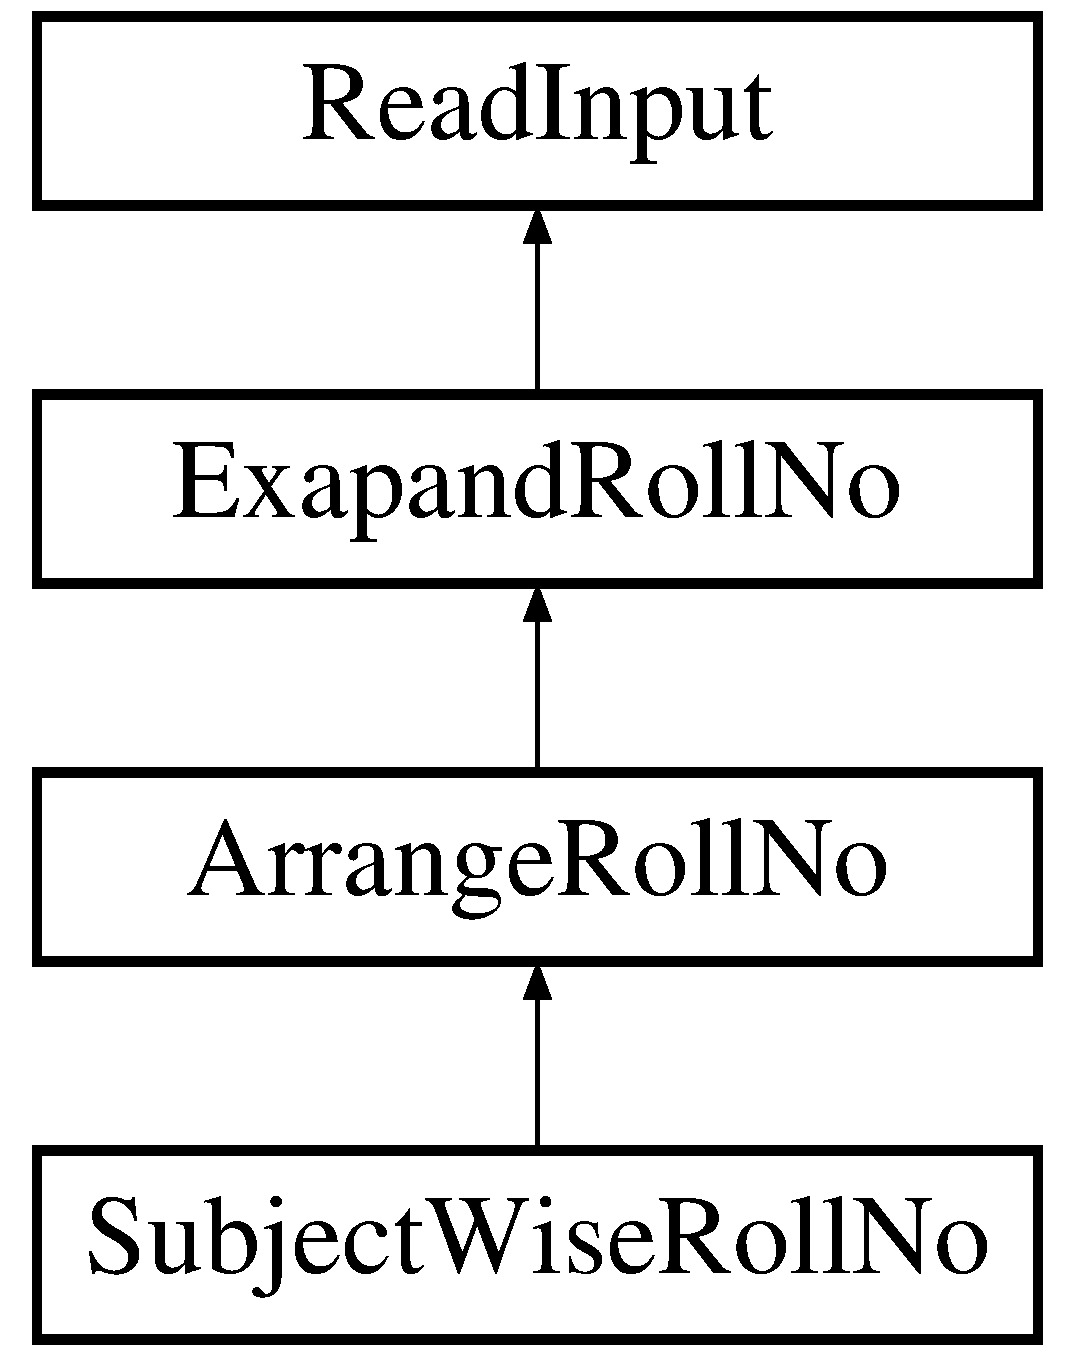
\includegraphics[height=3.000000cm]{classArrangeRollNo}
\end{center}
\end{figure}
\subsection*{\-Public \-Member \-Functions}
\begin{DoxyCompactItemize}
\item 
\hyperlink{classArrangeRollNo_a430515990d97ffa02b65ed5d15d79c9f}{\-Arrange\-Roll\-No} ()
\begin{DoxyCompactList}\small\item\em \-Constructor. \end{DoxyCompactList}\item 
void \hyperlink{classArrangeRollNo_aae9734fb7b98d980d3f1feb1b52a6195}{\-Sort\-Roll\-No} (\-I\-N\-T\-\_\-\-V\-E\-C \&rollno)
\begin{DoxyCompactList}\small\item\em \-Function for sorting roll no vector array. \end{DoxyCompactList}\item 
void \hyperlink{classArrangeRollNo_ab0b6350a9113b86925133d7199929020}{\-Remove\-Redundancy} (\-I\-N\-T\-\_\-\-V\-E\-C \&rollno)
\item 
void \hyperlink{classArrangeRollNo_adeb652c1977c668d2cd519c1a4f317bd}{\-Remove\-Non\-Eligible\-Roll\-No} (\-I\-N\-T\-\_\-\-V\-E\-C \&rollno, \-I\-N\-T\-\_\-\-V\-E\-C \&\hyperlink{classArrangeRollNo_a1f6740950e3180731b74c3ecdc19b98c}{not\-Included\-R\-No})
\begin{DoxyCompactList}\small\item\em \-Removing roll no that are not eligible. \end{DoxyCompactList}\item 
void \hyperlink{classArrangeRollNo_a69151212acbfeb90780b066ade988418}{\-Add\-Prefix\-With\-Roll\-No} (\-I\-N\-T\-\_\-\-V\-E\-C \&rollno, \-S\-T\-R\-I\-N\-G\-\_\-\-V\-E\-C \&\hyperlink{classArrangeRollNo_ac70b1f6e601cc5786ef339a38ae18c6f}{prefix})
\begin{DoxyCompactList}\small\item\em \-Adding prefix with roll nos. \end{DoxyCompactList}\item 
void \hyperlink{classArrangeRollNo_a12e17989e12519e37083b7f5649ebbec}{\-Write\-Arranged\-Roll\-No} ()
\begin{DoxyCompactList}\small\item\em \-Writing arranged roll nos to file as \-O/p file. \end{DoxyCompactList}\item 
void \hyperlink{classArrangeRollNo_a795fde3b512631e07d7189138b39b775}{\-Main} (string p\-I\-D)
\begin{DoxyCompactList}\small\item\em \-Main function to call all functions. \end{DoxyCompactList}\item 
\hyperlink{classArrangeRollNo_acbdaa06590d381ec19a7a07c718b9282}{$\sim$\-Arrange\-Roll\-No} ()
\begin{DoxyCompactList}\small\item\em \-Destructor. \end{DoxyCompactList}\end{DoxyCompactItemize}
\subsection*{\-Protected \-Attributes}
\begin{DoxyCompactItemize}
\item 
\-I\-N\-T\-\_\-\-V\-E\-C \hyperlink{classArrangeRollNo_ad75d3ee3f709606da5b4871098c3e978}{roll\-No}
\item 
\-I\-N\-T\-\_\-\-V\-E\-C \hyperlink{classArrangeRollNo_a1f6740950e3180731b74c3ecdc19b98c}{not\-Included\-R\-No}
\item 
\hypertarget{classArrangeRollNo_ab39f82c658365388d106b3dcc18e69fb}{\-I\-N\-T\-\_\-\-V\-E\-C {\bfseries roll\-No\-Size}}\label{classArrangeRollNo_ab39f82c658365388d106b3dcc18e69fb}

\item 
\hypertarget{classArrangeRollNo_a728b87c54815f5393e93da5909ed90b2}{\-I\-N\-T\-\_\-\-V\-E\-C {\bfseries not\-Included\-R\-No\-Size}}\label{classArrangeRollNo_a728b87c54815f5393e93da5909ed90b2}

\item 
\-S\-T\-R\-I\-N\-G\-\_\-\-V\-E\-C \hyperlink{classArrangeRollNo_ac70b1f6e601cc5786ef339a38ae18c6f}{prefix}
\item 
\-S\-T\-R\-I\-N\-G\-\_\-2\-D\-V\-E\-C \hyperlink{classArrangeRollNo_aa0401159b5d59c7afe77980a391a9a0a}{prefix\-Roll\-No}
\item 
\hyperlink{classExpandRollNo}{\-Expand\-Roll\-No} \hyperlink{classArrangeRollNo_a7ddd59b57f85cf6fea265d38c284df92}{expand\-R\-No}
\end{DoxyCompactItemize}


\subsection{\-Detailed \-Description}
\-Arrange roll no class for sorting, removing redundant roll nos and also excludeing roll nos that are not for seating plan. 

\-Include \hyperlink{arrangerollno_8h}{arrangerollno.\-h} file

\-Include \hyperlink{expandrollno_8h}{expandrollno.\-h} file 

\-Definition at line 30 of file arrangerollno.\-h.



\subsection{\-Constructor \& \-Destructor \-Documentation}
\hypertarget{classArrangeRollNo_a430515990d97ffa02b65ed5d15d79c9f}{\index{\-Arrange\-Roll\-No@{\-Arrange\-Roll\-No}!\-Arrange\-Roll\-No@{\-Arrange\-Roll\-No}}
\index{\-Arrange\-Roll\-No@{\-Arrange\-Roll\-No}!ArrangeRollNo@{\-Arrange\-Roll\-No}}
\subsubsection[{\-Arrange\-Roll\-No}]{\setlength{\rightskip}{0pt plus 5cm}{\bf \-Arrange\-Roll\-No\-::\-Arrange\-Roll\-No} (
\begin{DoxyParamCaption}
{}
\end{DoxyParamCaption}
)}}\label{classArrangeRollNo_a430515990d97ffa02b65ed5d15d79c9f}


\-Constructor. 

\-Constructor 

\-Definition at line 27 of file arrangerollno.\-cc.

\hypertarget{classArrangeRollNo_acbdaa06590d381ec19a7a07c718b9282}{\index{\-Arrange\-Roll\-No@{\-Arrange\-Roll\-No}!$\sim$\-Arrange\-Roll\-No@{$\sim$\-Arrange\-Roll\-No}}
\index{$\sim$\-Arrange\-Roll\-No@{$\sim$\-Arrange\-Roll\-No}!ArrangeRollNo@{\-Arrange\-Roll\-No}}
\subsubsection[{$\sim$\-Arrange\-Roll\-No}]{\setlength{\rightskip}{0pt plus 5cm}{\bf \-Arrange\-Roll\-No\-::$\sim$\-Arrange\-Roll\-No} (
\begin{DoxyParamCaption}
{}
\end{DoxyParamCaption}
)}}\label{classArrangeRollNo_acbdaa06590d381ec19a7a07c718b9282}


\-Destructor. 

\-Desrtuctor 

\-Definition at line 212 of file arrangerollno.\-cc.



\subsection{\-Member \-Function \-Documentation}
\hypertarget{classArrangeRollNo_a69151212acbfeb90780b066ade988418}{\index{\-Arrange\-Roll\-No@{\-Arrange\-Roll\-No}!\-Add\-Prefix\-With\-Roll\-No@{\-Add\-Prefix\-With\-Roll\-No}}
\index{\-Add\-Prefix\-With\-Roll\-No@{\-Add\-Prefix\-With\-Roll\-No}!ArrangeRollNo@{\-Arrange\-Roll\-No}}
\subsubsection[{\-Add\-Prefix\-With\-Roll\-No}]{\setlength{\rightskip}{0pt plus 5cm}void {\bf \-Arrange\-Roll\-No\-::\-Add\-Prefix\-With\-Roll\-No} (
\begin{DoxyParamCaption}
\item[{\-I\-N\-T\-\_\-\-V\-E\-C \&}]{roll\-No, }
\item[{\-S\-T\-R\-I\-N\-G\-\_\-\-V\-E\-C \&}]{prefix}
\end{DoxyParamCaption}
)}}\label{classArrangeRollNo_a69151212acbfeb90780b066ade988418}


\-Adding prefix with roll nos. 

\-Adding prefix with roll nos


\begin{DoxyParams}{\-Parameters}
{\em roll\-No} & \-List of eligible roll nos \\
\hline
{\em prefix} & \-Prefix ie added with roll nos \\
\hline
\end{DoxyParams}


\-Definition at line 107 of file arrangerollno.\-cc.

\hypertarget{classArrangeRollNo_a795fde3b512631e07d7189138b39b775}{\index{\-Arrange\-Roll\-No@{\-Arrange\-Roll\-No}!\-Main@{\-Main}}
\index{\-Main@{\-Main}!ArrangeRollNo@{\-Arrange\-Roll\-No}}
\subsubsection[{\-Main}]{\setlength{\rightskip}{0pt plus 5cm}void {\bf \-Arrange\-Roll\-No\-::\-Main} (
\begin{DoxyParamCaption}
\item[{string}]{p\-I\-D}
\end{DoxyParamCaption}
)}}\label{classArrangeRollNo_a795fde3b512631e07d7189138b39b775}


\-Main function to call all functions. 

\-Main method to call all function in order/sequence


\begin{DoxyParams}{\-Parameters}
{\em p\-I\-D} & \-Project \-I\-D \\
\hline
\end{DoxyParams}


\-Reimplemented in \hyperlink{classDateSheet_af749306c14297b5c93c16f48f551d5bb}{\-Date\-Sheet}.



\-Definition at line 151 of file arrangerollno.\-cc.

\hypertarget{classArrangeRollNo_adeb652c1977c668d2cd519c1a4f317bd}{\index{\-Arrange\-Roll\-No@{\-Arrange\-Roll\-No}!\-Remove\-Non\-Eligible\-Roll\-No@{\-Remove\-Non\-Eligible\-Roll\-No}}
\index{\-Remove\-Non\-Eligible\-Roll\-No@{\-Remove\-Non\-Eligible\-Roll\-No}!ArrangeRollNo@{\-Arrange\-Roll\-No}}
\subsubsection[{\-Remove\-Non\-Eligible\-Roll\-No}]{\setlength{\rightskip}{0pt plus 5cm}void {\bf \-Arrange\-Roll\-No\-::\-Remove\-Non\-Eligible\-Roll\-No} (
\begin{DoxyParamCaption}
\item[{\-I\-N\-T\-\_\-\-V\-E\-C \&}]{roll\-No, }
\item[{\-I\-N\-T\-\_\-\-V\-E\-C \&}]{not\-Included\-R\-No}
\end{DoxyParamCaption}
)}}\label{classArrangeRollNo_adeb652c1977c668d2cd519c1a4f317bd}


\-Removing roll no that are not eligible. 

\-Removing non eligible roll nos


\begin{DoxyParams}{\-Parameters}
{\em roll\-No} & roll nos for seating plan \\
\hline
{\em not\-Included\-R\-No} & \-Roll no list that is not eligible for seating plan \\
\hline
\end{DoxyParams}


\-Definition at line 79 of file arrangerollno.\-cc.

\hypertarget{classArrangeRollNo_ab0b6350a9113b86925133d7199929020}{\index{\-Arrange\-Roll\-No@{\-Arrange\-Roll\-No}!\-Remove\-Redundancy@{\-Remove\-Redundancy}}
\index{\-Remove\-Redundancy@{\-Remove\-Redundancy}!ArrangeRollNo@{\-Arrange\-Roll\-No}}
\subsubsection[{\-Remove\-Redundancy}]{\setlength{\rightskip}{0pt plus 5cm}void {\bf \-Arrange\-Roll\-No\-::\-Remove\-Redundancy} (
\begin{DoxyParamCaption}
\item[{\-I\-N\-T\-\_\-\-V\-E\-C \&}]{rollno}
\end{DoxyParamCaption}
)}}\label{classArrangeRollNo_ab0b6350a9113b86925133d7199929020}
\-Removing redundancy from roll nos 

\-Definition at line 51 of file arrangerollno.\-cc.

\hypertarget{classArrangeRollNo_aae9734fb7b98d980d3f1feb1b52a6195}{\index{\-Arrange\-Roll\-No@{\-Arrange\-Roll\-No}!\-Sort\-Roll\-No@{\-Sort\-Roll\-No}}
\index{\-Sort\-Roll\-No@{\-Sort\-Roll\-No}!ArrangeRollNo@{\-Arrange\-Roll\-No}}
\subsubsection[{\-Sort\-Roll\-No}]{\setlength{\rightskip}{0pt plus 5cm}void {\bf \-Arrange\-Roll\-No\-::\-Sort\-Roll\-No} (
\begin{DoxyParamCaption}
\item[{\-I\-N\-T\-\_\-\-V\-E\-C \&}]{roll\-No}
\end{DoxyParamCaption}
)}}\label{classArrangeRollNo_aae9734fb7b98d980d3f1feb1b52a6195}


\-Function for sorting roll no vector array. 

\-Sorting \-Roll nos


\begin{DoxyParams}{\-Parameters}
{\em roll\-No} & \-For sorting array \\
\hline
\end{DoxyParams}


\-Definition at line 39 of file arrangerollno.\-cc.

\hypertarget{classArrangeRollNo_a12e17989e12519e37083b7f5649ebbec}{\index{\-Arrange\-Roll\-No@{\-Arrange\-Roll\-No}!\-Write\-Arranged\-Roll\-No@{\-Write\-Arranged\-Roll\-No}}
\index{\-Write\-Arranged\-Roll\-No@{\-Write\-Arranged\-Roll\-No}!ArrangeRollNo@{\-Arrange\-Roll\-No}}
\subsubsection[{\-Write\-Arranged\-Roll\-No}]{\setlength{\rightskip}{0pt plus 5cm}void {\bf \-Arrange\-Roll\-No\-::\-Write\-Arranged\-Roll\-No} (
\begin{DoxyParamCaption}
{}
\end{DoxyParamCaption}
)}}\label{classArrangeRollNo_a12e17989e12519e37083b7f5649ebbec}


\-Writing arranged roll nos to file as \-O/p file. 

\-Writing arranged roll no's into file 

\-Definition at line 124 of file arrangerollno.\-cc.



\subsection{\-Member \-Data \-Documentation}
\hypertarget{classArrangeRollNo_a7ddd59b57f85cf6fea265d38c284df92}{\index{\-Arrange\-Roll\-No@{\-Arrange\-Roll\-No}!expand\-R\-No@{expand\-R\-No}}
\index{expand\-R\-No@{expand\-R\-No}!ArrangeRollNo@{\-Arrange\-Roll\-No}}
\subsubsection[{expand\-R\-No}]{\setlength{\rightskip}{0pt plus 5cm}{\bf \-Expand\-Roll\-No} {\bf \-Arrange\-Roll\-No\-::expand\-R\-No}\hspace{0.3cm}{\ttfamily  \mbox{[}protected\mbox{]}}}}\label{classArrangeRollNo_a7ddd59b57f85cf6fea265d38c284df92}
\-Object of \hyperlink{classExpandRollNo}{\-Expand\-Roll\-No} class 

\-Definition at line 45 of file arrangerollno.\-h.

\hypertarget{classArrangeRollNo_a1f6740950e3180731b74c3ecdc19b98c}{\index{\-Arrange\-Roll\-No@{\-Arrange\-Roll\-No}!not\-Included\-R\-No@{not\-Included\-R\-No}}
\index{not\-Included\-R\-No@{not\-Included\-R\-No}!ArrangeRollNo@{\-Arrange\-Roll\-No}}
\subsubsection[{not\-Included\-R\-No}]{\setlength{\rightskip}{0pt plus 5cm}\-I\-N\-T\-\_\-\-V\-E\-C {\bf \-Arrange\-Roll\-No\-::not\-Included\-R\-No}\hspace{0.3cm}{\ttfamily  \mbox{[}protected\mbox{]}}}}\label{classArrangeRollNo_a1f6740950e3180731b74c3ecdc19b98c}
stroring rollnos that are not included 

\-Definition at line 34 of file arrangerollno.\-h.

\hypertarget{classArrangeRollNo_ac70b1f6e601cc5786ef339a38ae18c6f}{\index{\-Arrange\-Roll\-No@{\-Arrange\-Roll\-No}!prefix@{prefix}}
\index{prefix@{prefix}!ArrangeRollNo@{\-Arrange\-Roll\-No}}
\subsubsection[{prefix}]{\setlength{\rightskip}{0pt plus 5cm}\-S\-T\-R\-I\-N\-G\-\_\-\-V\-E\-C {\bf \-Arrange\-Roll\-No\-::prefix}\hspace{0.3cm}{\ttfamily  \mbox{[}protected\mbox{]}}}}\label{classArrangeRollNo_ac70b1f6e601cc5786ef339a38ae18c6f}
\-Storing prefix of roll nos 

\-Reimplemented from \hyperlink{classReadInput_a6a96c934f8c9a2a2056dc50505017e52}{\-Read\-Input}.



\-Definition at line 40 of file arrangerollno.\-h.

\hypertarget{classArrangeRollNo_aa0401159b5d59c7afe77980a391a9a0a}{\index{\-Arrange\-Roll\-No@{\-Arrange\-Roll\-No}!prefix\-Roll\-No@{prefix\-Roll\-No}}
\index{prefix\-Roll\-No@{prefix\-Roll\-No}!ArrangeRollNo@{\-Arrange\-Roll\-No}}
\subsubsection[{prefix\-Roll\-No}]{\setlength{\rightskip}{0pt plus 5cm}\-S\-T\-R\-I\-N\-G\-\_\-2\-D\-V\-E\-C {\bf \-Arrange\-Roll\-No\-::prefix\-Roll\-No}\hspace{0.3cm}{\ttfamily  \mbox{[}protected\mbox{]}}}}\label{classArrangeRollNo_aa0401159b5d59c7afe77980a391a9a0a}
\-Roll no with prefix 

\-Definition at line 43 of file arrangerollno.\-h.

\hypertarget{classArrangeRollNo_ad75d3ee3f709606da5b4871098c3e978}{\index{\-Arrange\-Roll\-No@{\-Arrange\-Roll\-No}!roll\-No@{roll\-No}}
\index{roll\-No@{roll\-No}!ArrangeRollNo@{\-Arrange\-Roll\-No}}
\subsubsection[{roll\-No}]{\setlength{\rightskip}{0pt plus 5cm}\-I\-N\-T\-\_\-\-V\-E\-C {\bf \-Arrange\-Roll\-No\-::roll\-No}\hspace{0.3cm}{\ttfamily  \mbox{[}protected\mbox{]}}}}\label{classArrangeRollNo_ad75d3ee3f709606da5b4871098c3e978}
\-Reading roll nos 

\-Reimplemented from \hyperlink{classReadInput_a862fbffdffa56fc6d66b1d1f14dae087}{\-Read\-Input}.



\-Definition at line 34 of file arrangerollno.\-h.



\-The documentation for this class was generated from the following files\-:\begin{DoxyCompactItemize}
\item 
frontend/src/backend/header/\hyperlink{arrangerollno_8h}{arrangerollno.\-h}\item 
frontend/src/backend/\hyperlink{arrangerollno_8cc}{arrangerollno.\-cc}\end{DoxyCompactItemize}

\hypertarget{classBranchReport}{\section{Branch\-Report Class Reference}
\label{classBranchReport}\index{Branch\-Report@{Branch\-Report}}
}
Inheritance diagram for Branch\-Report\-:\begin{figure}[H]
\begin{center}
\leavevmode
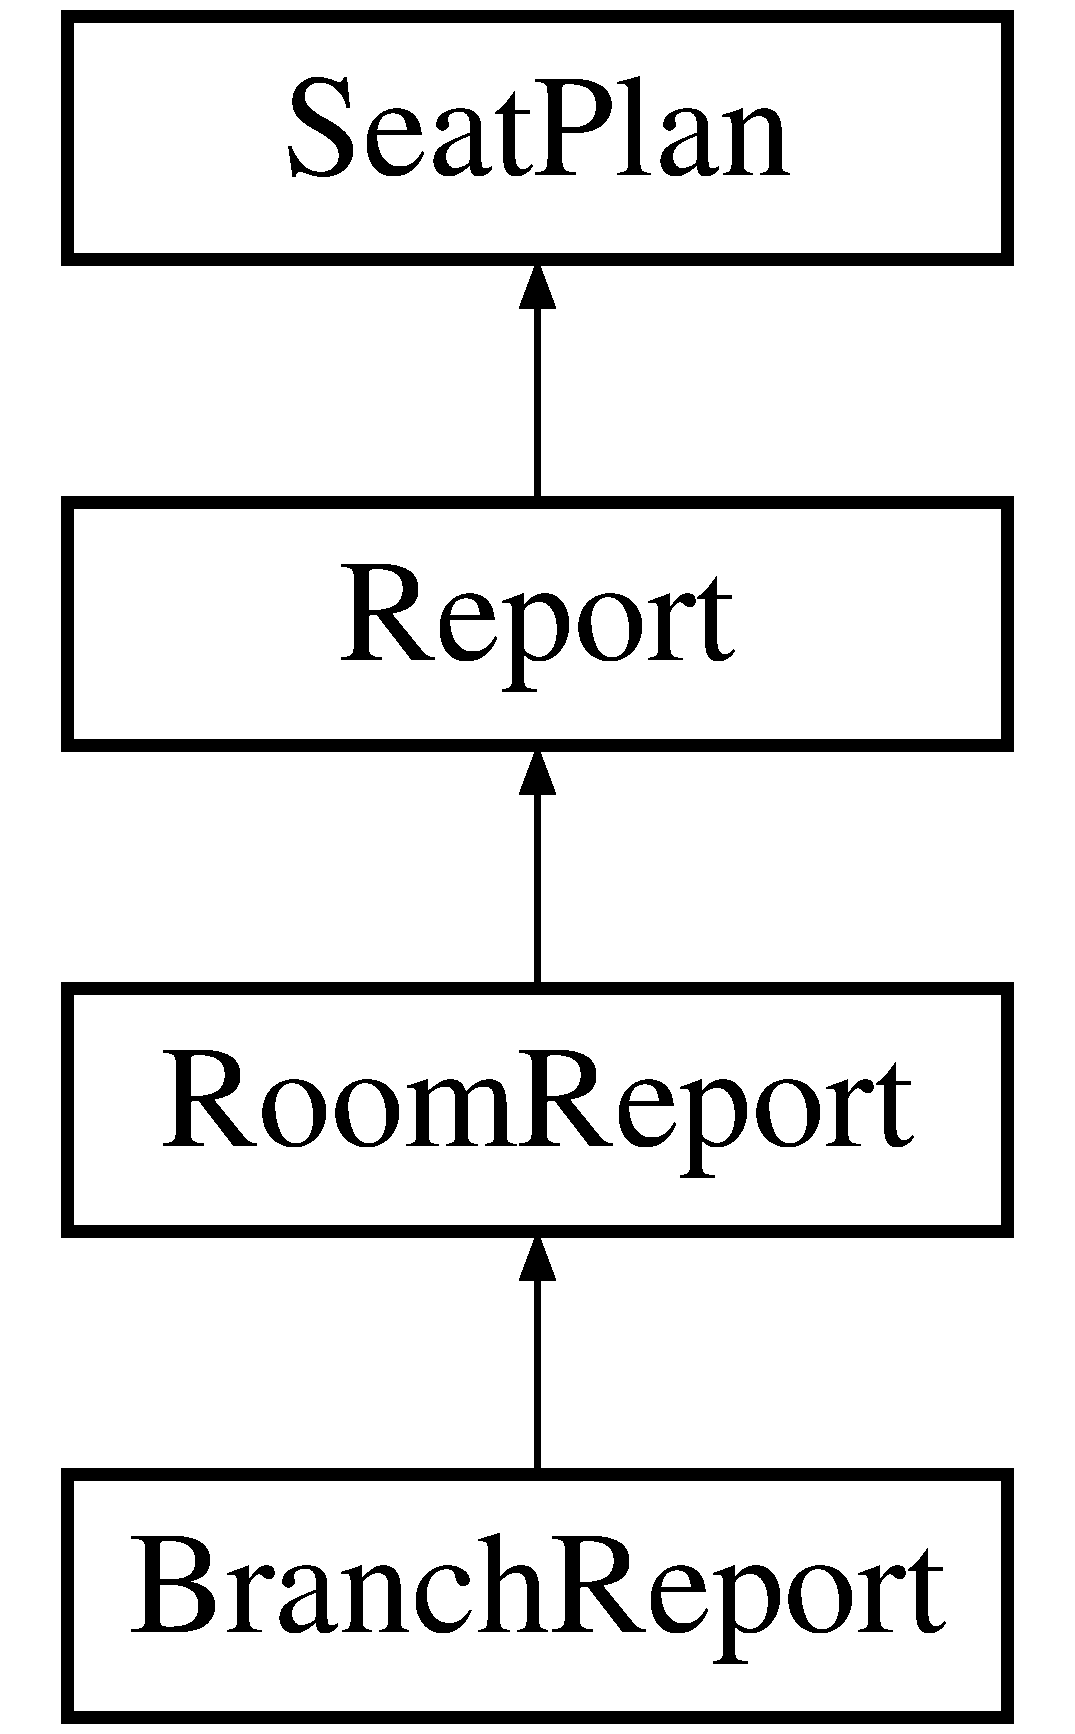
\includegraphics[height=3.000000cm]{classBranchReport}
\end{center}
\end{figure}
\subsection*{Public Member Functions}
\begin{DoxyCompactItemize}
\item 
\hypertarget{classBranchReport_acafa37b5ff6b8886333cc5ab8bb53fad}{void {\bfseries Main} ()}\label{classBranchReport_acafa37b5ff6b8886333cc5ab8bb53fad}

\end{DoxyCompactItemize}
\subsection*{Additional Inherited Members}


The documentation for this class was generated from the following file\-:\begin{DoxyCompactItemize}
\item 
Baka\-Plan/\-Seat\-Plan/report.\-h\end{DoxyCompactItemize}

\hypertarget{classExapandRollNo}{\section{Exapand\-Roll\-No Class Reference}
\label{classExapandRollNo}\index{Exapand\-Roll\-No@{Exapand\-Roll\-No}}
}
Inheritance diagram for Exapand\-Roll\-No\-:\begin{figure}[H]
\begin{center}
\leavevmode
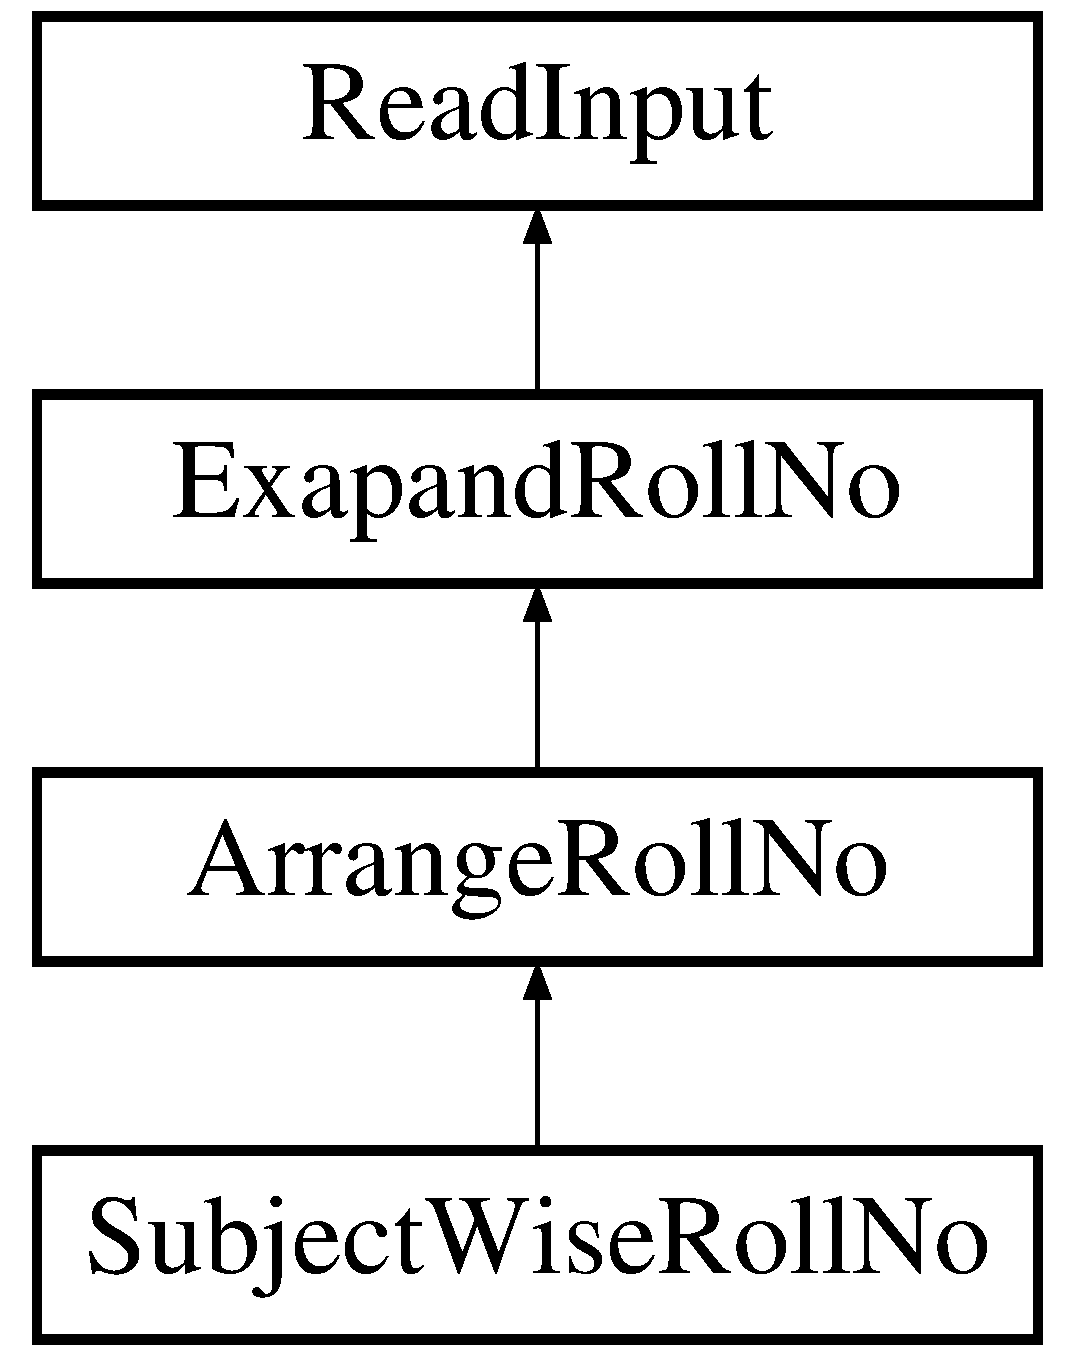
\includegraphics[height=4.000000cm]{classExapandRollNo}
\end{center}
\end{figure}
\subsection*{Public Member Functions}
\begin{DoxyCompactItemize}
\item 
\hypertarget{classExapandRollNo_a19a299d6ebbff3af32fdee08fcc164ee}{void {\bfseries expand\-Input} ()}\label{classExapandRollNo_a19a299d6ebbff3af32fdee08fcc164ee}

\item 
\hypertarget{classExapandRollNo_ad1a2a298aa0834a6da672e152cd4e24f}{void {\bfseries add\-Seperator} ()}\label{classExapandRollNo_ad1a2a298aa0834a6da672e152cd4e24f}

\item 
\hypertarget{classExapandRollNo_a9125b4dc6bbdb81dc4007cec1e86a7e9}{void {\bfseries expand\-Roll\-No} ()}\label{classExapandRollNo_a9125b4dc6bbdb81dc4007cec1e86a7e9}

\item 
\hypertarget{classExapandRollNo_a69ff3dc919a8b297b46926839184b349}{{\footnotesize template$<$typename Out\-Iter $>$ }\\bool {\bfseries expand\-Roll\-Number\-List} (istream \&is, Out\-Iter out)}\label{classExapandRollNo_a69ff3dc919a8b297b46926839184b349}

\item 
\hypertarget{classExapandRollNo_a3b767bfce279771a398abaa725753e33}{void {\bfseries remove\-Zero} ()}\label{classExapandRollNo_a3b767bfce279771a398abaa725753e33}

\item 
\hypertarget{classExapandRollNo_ae11d041a516d6fce629364d6e6796955}{void {\bfseries show\-Expand\-Roll\-No} ()}\label{classExapandRollNo_ae11d041a516d6fce629364d6e6796955}

\item 
\hypertarget{classExapandRollNo_afbfccde139eb71155e0b0fce02962d1c}{void {\bfseries Main} ()}\label{classExapandRollNo_afbfccde139eb71155e0b0fce02962d1c}

\end{DoxyCompactItemize}
\subsection*{Protected Attributes}
\begin{DoxyCompactItemize}
\item 
\hypertarget{classExapandRollNo_ae27a8647cfc7f93a5ba2fbfef8afa5c8}{int {\bfseries roll\-\_\-no} \mbox{[}M\-I\-N\-\_\-\-S\-I\-Z\-E\mbox{]}\mbox{[}M\-A\-X\-\_\-\-S\-I\-Z\-E\mbox{]}\mbox{[}M\-A\-X\-\_\-\-S\-I\-Z\-E\mbox{]}}\label{classExapandRollNo_ae27a8647cfc7f93a5ba2fbfef8afa5c8}

\item 
\hypertarget{classExapandRollNo_a892479a25a021a95e9c4b38ed30208a5}{int {\bfseries roll\-\_\-size} \mbox{[}M\-I\-N\-\_\-\-S\-I\-Z\-E\mbox{]}\mbox{[}M\-I\-N\-\_\-\-S\-I\-Z\-E\mbox{]}}\label{classExapandRollNo_a892479a25a021a95e9c4b38ed30208a5}

\item 
\hypertarget{classExapandRollNo_ac3526c93e25b52ab118f66150c980dbd}{int {\bfseries not\-\_\-roll\-\_\-no} \mbox{[}M\-I\-N\-\_\-\-S\-I\-Z\-E\mbox{]}\mbox{[}M\-A\-X\-\_\-\-S\-I\-Z\-E\mbox{]}\mbox{[}M\-A\-X\-\_\-\-S\-I\-Z\-E\mbox{]}}\label{classExapandRollNo_ac3526c93e25b52ab118f66150c980dbd}

\item 
\hypertarget{classExapandRollNo_a809856dbd610c81509f2fdf2cc11e57f}{int {\bfseries not\-\_\-roll\-\_\-size} \mbox{[}M\-I\-N\-\_\-\-S\-I\-Z\-E\mbox{]}\mbox{[}M\-I\-N\-\_\-\-S\-I\-Z\-E\mbox{]}}\label{classExapandRollNo_a809856dbd610c81509f2fdf2cc11e57f}

\end{DoxyCompactItemize}


The documentation for this class was generated from the following files\-:\begin{DoxyCompactItemize}
\item 
expand-\/rollno.\-h\item 
expand-\/rollno.\-cc\end{DoxyCompactItemize}

\hypertarget{classReadInput}{\section{Read\-Input Class Reference}
\label{classReadInput}\index{Read\-Input@{Read\-Input}}
}


\subsection{Detailed Description}
Include readinput.\-h file 

The documentation for this class was generated from the following file\-:\begin{DoxyCompactItemize}
\item 
frontend/src/backend/\hyperlink{readinput_8cc}{readinput.\-cc}\end{DoxyCompactItemize}

\hypertarget{classReport}{\section{Report Class Reference}
\label{classReport}\index{Report@{Report}}
}
Inheritance diagram for Report\-:\begin{figure}[H]
\begin{center}
\leavevmode
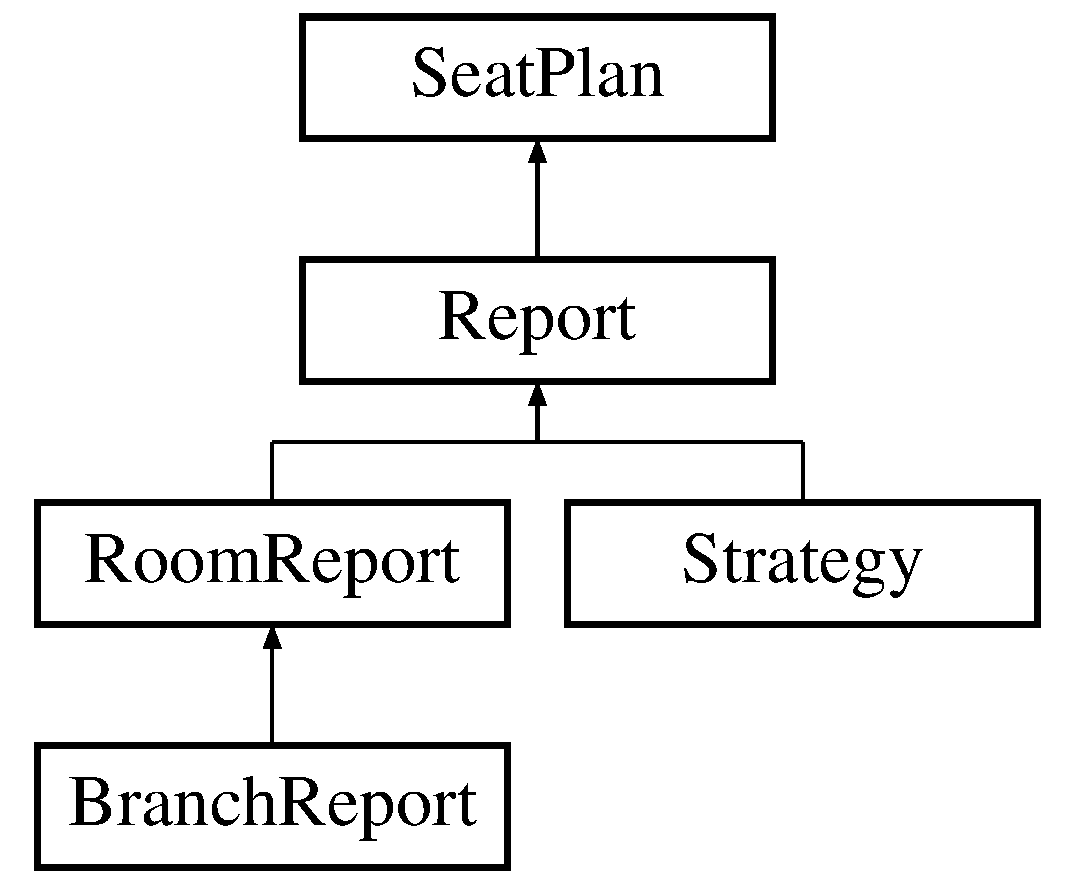
\includegraphics[height=3.000000cm]{classReport}
\end{center}
\end{figure}
\subsection*{Public Member Functions}
\begin{DoxyCompactItemize}
\item 
\hypertarget{classReport_a6b5a749dcbc19cb71503c5a6e2d465d3}{void {\bfseries Head} ()}\label{classReport_a6b5a749dcbc19cb71503c5a6e2d465d3}

\item 
\hypertarget{classReport_a97998b106d6fb7d6ccfea849892d21ee}{void {\bfseries Javascript} ()}\label{classReport_a97998b106d6fb7d6ccfea849892d21ee}

\item 
\hypertarget{classReport_a28dfc98e680194276c2bbb2fa4decf86}{void {\bfseries Body} ()}\label{classReport_a28dfc98e680194276c2bbb2fa4decf86}

\item 
\hypertarget{classReport_abfacfc97c910b8c2bc1a1102cc623d80}{void {\bfseries Body\-Content} ()}\label{classReport_abfacfc97c910b8c2bc1a1102cc623d80}

\item 
\hypertarget{classReport_a35895231f3a27c3247f9498cda2b42fe}{void {\bfseries Main} ()}\label{classReport_a35895231f3a27c3247f9498cda2b42fe}

\end{DoxyCompactItemize}
\subsection*{Additional Inherited Members}


The documentation for this class was generated from the following files\-:\begin{DoxyCompactItemize}
\item 
Baka\-Plan/report.\-h\item 
Baka\-Plan/report.\-cc\end{DoxyCompactItemize}

\hypertarget{classRoomReport}{\section{Room\-Report Class Reference}
\label{classRoomReport}\index{Room\-Report@{Room\-Report}}
}
Inheritance diagram for Room\-Report\-:\begin{figure}[H]
\begin{center}
\leavevmode
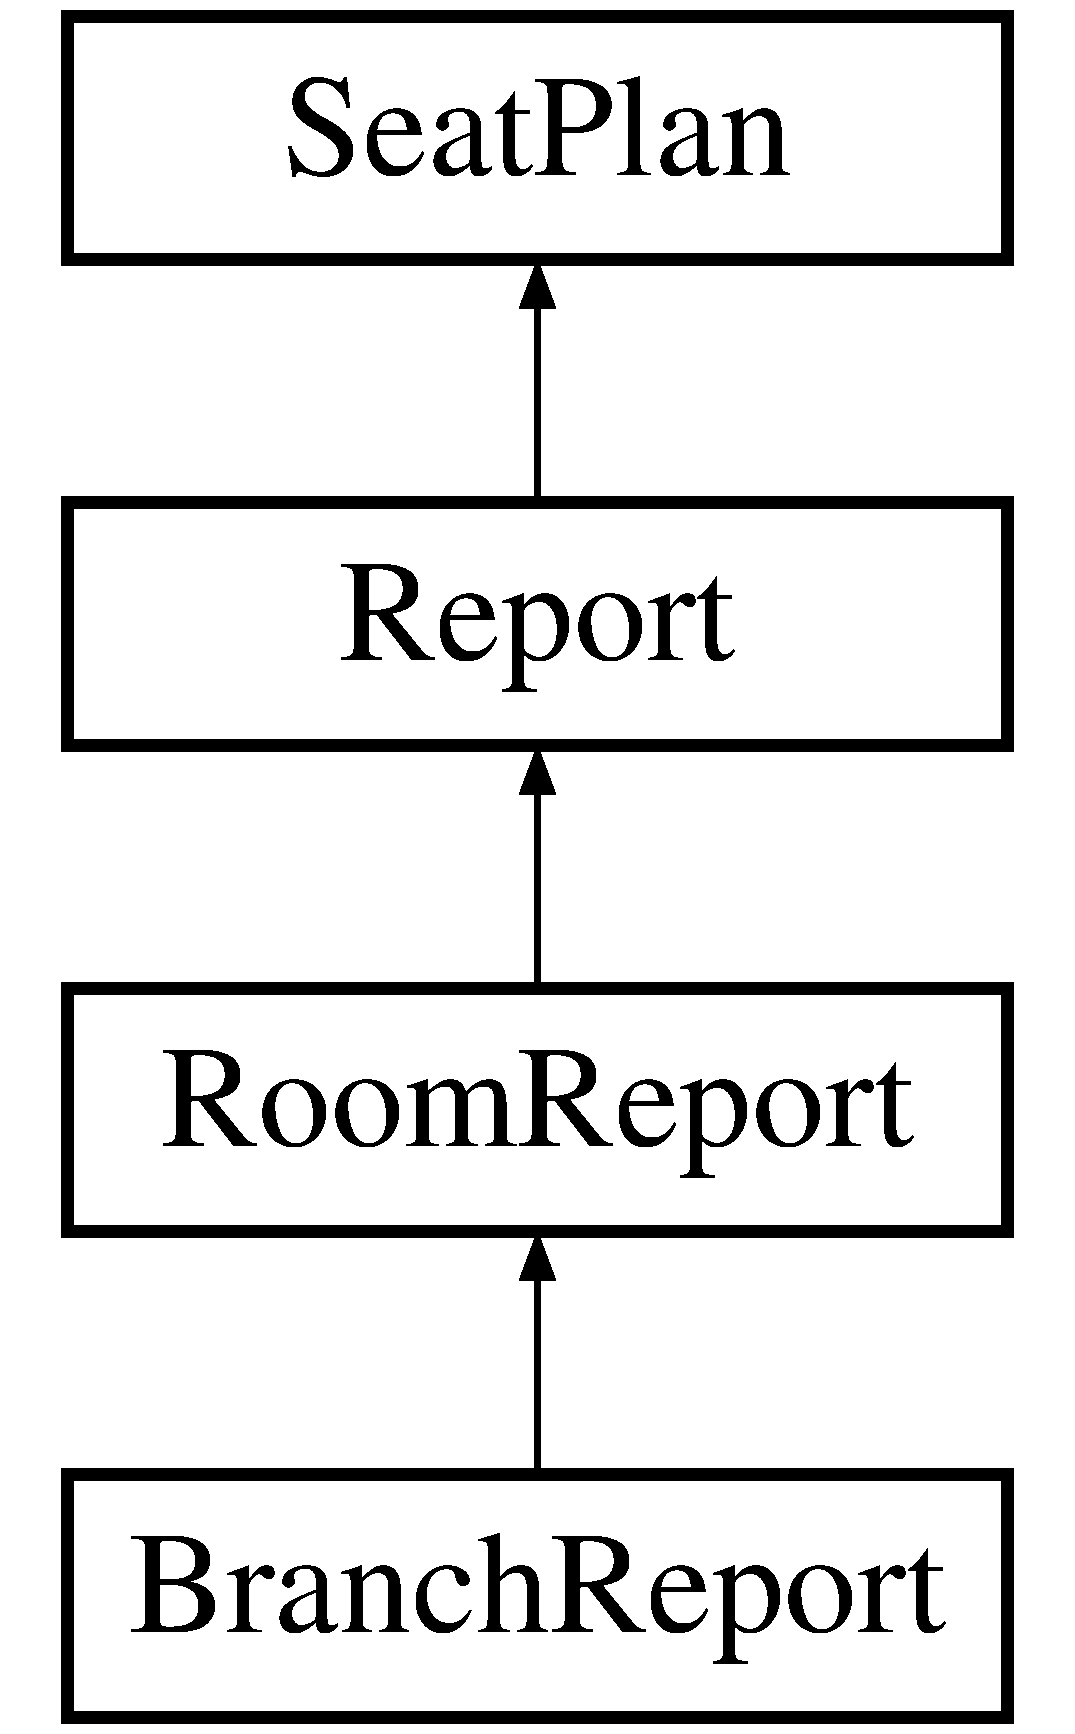
\includegraphics[height=3.000000cm]{classRoomReport}
\end{center}
\end{figure}
\subsection*{Public Member Functions}
\begin{DoxyCompactItemize}
\item 
\hypertarget{classRoomReport_a6befa64df45c74ac5d4810d3b0abdb2c}{void {\bfseries read\-Input\-Roll\-No} (string)}\label{classRoomReport_a6befa64df45c74ac5d4810d3b0abdb2c}

\item 
\hypertarget{classRoomReport_a488ef42cd98cf26383c5753af972dfde}{void {\bfseries read\-Seat\-Plan} (string)}\label{classRoomReport_a488ef42cd98cf26383c5753af972dfde}

\item 
\hypertarget{classRoomReport_a74d8d4a54ab1a80d84c059827ec3c4f6}{void {\bfseries read\-Exam\-Details} (string)}\label{classRoomReport_a74d8d4a54ab1a80d84c059827ec3c4f6}

\item 
\hypertarget{classRoomReport_a3704858e3ace6b7ef0104bdbecf745db}{void {\bfseries write\-Seat\-Plan} (string)}\label{classRoomReport_a3704858e3ace6b7ef0104bdbecf745db}

\item 
\hypertarget{classRoomReport_aa6eff185efa1c6205ec1446ed66d9766}{void {\bfseries Main} ()}\label{classRoomReport_aa6eff185efa1c6205ec1446ed66d9766}

\end{DoxyCompactItemize}
\subsection*{Protected Attributes}
\begin{DoxyCompactItemize}
\item 
\hypertarget{classRoomReport_af342c8a98e579b420ebde3783ad5f3df}{string {\bfseries rollno} \mbox{[}M\-I\-N\-\_\-\-S\-I\-Z\-E\mbox{]}\mbox{[}M\-I\-N\-\_\-\-S\-I\-Z\-E\mbox{]}\mbox{[}M\-A\-X\-\_\-\-S\-I\-Z\-E\mbox{]}}\label{classRoomReport_af342c8a98e579b420ebde3783ad5f3df}

\item 
\hypertarget{classRoomReport_a2582b819b47038641678e4645f25de34}{string {\bfseries branch\-\_\-name} \mbox{[}M\-I\-N\-\_\-\-S\-I\-Z\-E\mbox{]}}\label{classRoomReport_a2582b819b47038641678e4645f25de34}

\item 
\hypertarget{classRoomReport_a530a885bacdce429ae607b741216d4b5}{string {\bfseries subject\-\_\-name} \mbox{[}M\-I\-N\-\_\-\-S\-I\-Z\-E\mbox{]}\mbox{[}M\-I\-N\-\_\-\-S\-I\-Z\-E\mbox{]}}\label{classRoomReport_a530a885bacdce429ae607b741216d4b5}

\item 
\hypertarget{classRoomReport_a62207caf3dd352107bd2566138a98ae4}{string {\bfseries subject\-\_\-code} \mbox{[}M\-I\-N\-\_\-\-S\-I\-Z\-E\mbox{]}\mbox{[}M\-I\-N\-\_\-\-S\-I\-Z\-E\mbox{]}}\label{classRoomReport_a62207caf3dd352107bd2566138a98ae4}

\item 
\hypertarget{classRoomReport_a099a235828672ee6c31dd163d51e648c}{int {\bfseries total\-\_\-rollno} \mbox{[}M\-I\-N\-\_\-\-S\-I\-Z\-E\mbox{]}\mbox{[}M\-I\-N\-\_\-\-S\-I\-Z\-E\mbox{]}}\label{classRoomReport_a099a235828672ee6c31dd163d51e648c}

\item 
\hypertarget{classRoomReport_a4ce1c0593c6d5053575fcf7975ed1577}{int {\bfseries total\-\_\-branches}}\label{classRoomReport_a4ce1c0593c6d5053575fcf7975ed1577}

\item 
\hypertarget{classRoomReport_ad526976fbeecd9b4ad1888e1b90eb9ee}{int {\bfseries total\-\_\-subject} \mbox{[}M\-I\-N\-\_\-\-S\-I\-Z\-E\mbox{]}}\label{classRoomReport_ad526976fbeecd9b4ad1888e1b90eb9ee}

\end{DoxyCompactItemize}


The documentation for this class was generated from the following files\-:\begin{DoxyCompactItemize}
\item 
Baka\-Plan/\-Seat\-Plan/report.\-h\item 
Baka\-Plan/\-Seat\-Plan/room-\/report.\-cc\end{DoxyCompactItemize}

\hypertarget{classSeatPlan}{\section{Seat\-Plan Class Reference}
\label{classSeatPlan}\index{Seat\-Plan@{Seat\-Plan}}
}


\hyperlink{classSeatPlan}{Seat\-Plan} C\-Lass for generating seating plan.  




{\ttfamily \#include $<$report.\-h$>$}

Inheritance diagram for Seat\-Plan\-:\begin{figure}[H]
\begin{center}
\leavevmode
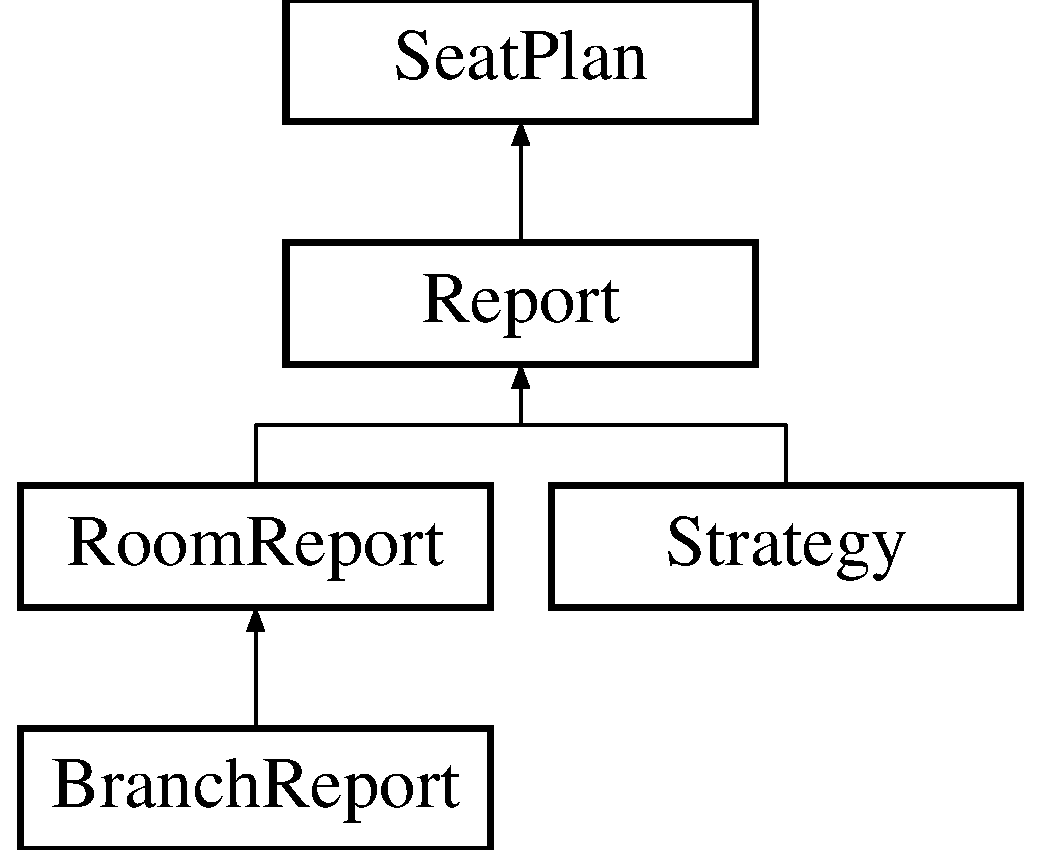
\includegraphics[height=3.000000cm]{classSeatPlan}
\end{center}
\end{figure}
\subsection*{Public Member Functions}
\begin{DoxyCompactItemize}
\item 
\hyperlink{classSeatPlan_a974a336df39c9fefc2b239a382a4749c}{Room\-Report} ()
\item 
void \hyperlink{classSeatPlan_ae93cefd4fd0401c5d54b8e97b23541ae}{Read\-Exam\-Detail} (string \hyperlink{classReadInput_a3ad470a25b3e0a29466bf4ff1f7d8e81}{project\-I\-D})
\item 
void \hyperlink{classSeatPlan_a618d148beefee9d4db3d038328c9b2c8}{Read\-Seat\-Plan} (string \hyperlink{classReadInput_a3ad470a25b3e0a29466bf4ff1f7d8e81}{project\-I\-D})
\item 
void \hyperlink{classSeatPlan_af572f79142f4dad362f54892c6747214}{Write\-H\-T\-M\-L\-File} (string \hyperlink{classReadInput_a3ad470a25b3e0a29466bf4ff1f7d8e81}{project\-I\-D})
\item 
\hyperlink{classSeatPlan_a446949506a25bcda5eb972c8a4b1384d}{$\sim$\-Room\-Report} ()
\item 
\hyperlink{classSeatPlan_ab1906186f96847704ed71f1a6c738327}{Seat\-Plan} ()
\begin{DoxyCompactList}\small\item\em Constructor. \end{DoxyCompactList}\item 
\hypertarget{classSeatPlan_afa418b9edadff831c73ea6005666becf}{void {\bfseries Set\-Roll\-No} (int strategy, int i)}\label{classSeatPlan_afa418b9edadff831c73ea6005666becf}

\item 
\hypertarget{classSeatPlan_a3dfc44c97eab7f3d33f2023ae0faaa13}{string {\bfseries Roll\-No} (int s)}\label{classSeatPlan_a3dfc44c97eab7f3d33f2023ae0faaa13}

\item 
\hypertarget{classSeatPlan_a1df3b03c983936c07225ed1a79959f1b}{void {\bfseries Seating\-Plan} (int strategy, int i)}\label{classSeatPlan_a1df3b03c983936c07225ed1a79959f1b}

\item 
\hypertarget{classSeatPlan_ade684c0f63b648d4d62df8e7ed800682}{void {\bfseries Create\-File} (string \hyperlink{classReadInput_a3ad470a25b3e0a29466bf4ff1f7d8e81}{project\-I\-D})}\label{classSeatPlan_ade684c0f63b648d4d62df8e7ed800682}

\item 
\hypertarget{classSeatPlan_a3f29cad9d9be46f7bc3055de2ab887fc}{void {\bfseries Write\-Seat\-Plan} (string \hyperlink{classReadInput_a3ad470a25b3e0a29466bf4ff1f7d8e81}{project\-I\-D}, int i)}\label{classSeatPlan_a3f29cad9d9be46f7bc3055de2ab887fc}

\item 
void \hyperlink{classSeatPlan_a67c10e2277f1f2823581cddf4df373c5}{Write\-H\-T\-M\-L\-File} (string \hyperlink{classReadInput_a3ad470a25b3e0a29466bf4ff1f7d8e81}{project\-I\-D}, int i)
\begin{DoxyCompactList}\small\item\em Creating H\-T\-M\-L file. \end{DoxyCompactList}\item 
\hypertarget{classSeatPlan_abce0c5b5545f1bb1ebcf2e578b6ab282}{void {\bfseries Write\-P\-D\-F\-File} (string \hyperlink{classReadInput_a3ad470a25b3e0a29466bf4ff1f7d8e81}{project\-I\-D}, int i)}\label{classSeatPlan_abce0c5b5545f1bb1ebcf2e578b6ab282}

\item 
\hypertarget{classSeatPlan_a3257eb25ac9c82d2757d2a7144614762}{void {\bfseries Add\-Roll\-No\-Info} (string \hyperlink{classReadInput_a3ad470a25b3e0a29466bf4ff1f7d8e81}{project\-I\-D}, int i)}\label{classSeatPlan_a3257eb25ac9c82d2757d2a7144614762}

\item 
\hyperlink{classSeatPlan_a373a1d60b6617a2e424f7d2f8866ec2e}{$\sim$\-Seat\-Plan} ()
\begin{DoxyCompactList}\small\item\em D\-Estructor. \end{DoxyCompactList}\end{DoxyCompactItemize}
\subsection*{Protected Attributes}
\begin{DoxyCompactItemize}
\item 
\hypertarget{classSeatPlan_a6915f74be45af73cda8c9a51b6cb99c9}{int {\bfseries total\-Seats}}\label{classSeatPlan_a6915f74be45af73cda8c9a51b6cb99c9}

\item 
\hypertarget{classSeatPlan_a3568dfc375740fd6b4075d7dc419a2e5}{int {\bfseries total\-Students}}\label{classSeatPlan_a3568dfc375740fd6b4075d7dc419a2e5}

\item 
\hypertarget{classSeatPlan_a18b1d6497343d6a9e751159dcdd8a179}{int {\bfseries total\-Group\-Seats}}\label{classSeatPlan_a18b1d6497343d6a9e751159dcdd8a179}

\item 
\hypertarget{classSeatPlan_acf6fa47342ec7f5675064c5601800f5c}{int {\bfseries day}}\label{classSeatPlan_acf6fa47342ec7f5675064c5601800f5c}

\item 
\hypertarget{classSeatPlan_a19a423aff33092a242f5dff5694efa37}{I\-N\-T\-\_\-\-V\-E\-C {\bfseries i\-Temp}}\label{classSeatPlan_a19a423aff33092a242f5dff5694efa37}

\item 
\hypertarget{classSeatPlan_af3fbce455c6744dee3fedb97442cd2c3}{I\-N\-T\-\_\-\-V\-E\-C {\bfseries index\-Value}}\label{classSeatPlan_af3fbce455c6744dee3fedb97442cd2c3}

\item 
\hypertarget{classSeatPlan_a6cb00329d2f0760f679d7e00958da879}{I\-N\-T\-\_\-\-V\-E\-C {\bfseries group\-Student\-Size}}\label{classSeatPlan_a6cb00329d2f0760f679d7e00958da879}

\item 
\hypertarget{classSeatPlan_a73de1d93e86c3a23406e0903c546ea2c}{I\-N\-T\-\_\-\-V\-E\-C {\bfseries seat\-Size}}\label{classSeatPlan_a73de1d93e86c3a23406e0903c546ea2c}

\item 
\hypertarget{classSeatPlan_a45d2c9c1d580d442bc15dcb50265d627}{I\-N\-T\-\_\-\-V\-E\-C {\bfseries size}}\label{classSeatPlan_a45d2c9c1d580d442bc15dcb50265d627}

\item 
\hypertarget{classSeatPlan_a52bafc6123bd54a8f95253c4693b2975}{I\-N\-T\-\_\-3\-D\-V\-E\-C {\bfseries room\-Size}}\label{classSeatPlan_a52bafc6123bd54a8f95253c4693b2975}

\item 
\hypertarget{classSeatPlan_ace374a7f84b7f9fb43fc56979a3793fb}{S\-T\-R\-I\-N\-G\-\_\-\-V\-E\-C {\bfseries sub\-Sub\-Code}}\label{classSeatPlan_ace374a7f84b7f9fb43fc56979a3793fb}

\item 
\hypertarget{classSeatPlan_adf8ed7579be4a43e20cbf4b40bb7b25e}{S\-T\-R\-I\-N\-G\-\_\-2\-D\-V\-E\-C {\bfseries seat\-Roll\-No}}\label{classSeatPlan_adf8ed7579be4a43e20cbf4b40bb7b25e}

\item 
\hypertarget{classSeatPlan_a38f161cde37bcfae5877a17f785cbb21}{S\-T\-R\-I\-N\-G\-\_\-2\-D\-V\-E\-C {\bfseries sub\-Roll\-No}}\label{classSeatPlan_a38f161cde37bcfae5877a17f785cbb21}

\item 
\hypertarget{classSeatPlan_a99f24fdf486af2b45bf142558011573d}{S\-T\-R\-I\-N\-G\-\_\-4\-D\-V\-E\-C {\bfseries seat}}\label{classSeatPlan_a99f24fdf486af2b45bf142558011573d}

\item 
\hypertarget{classSeatPlan_ac623e253b6005a0907c2dab61705f2ab}{int {\bfseries text\-Width}}\label{classSeatPlan_ac623e253b6005a0907c2dab61705f2ab}

\item 
\hypertarget{classSeatPlan_a2e67c39e7c6fff250ce3dc727f0680fd}{int {\bfseries text\-Width1}}\label{classSeatPlan_a2e67c39e7c6fff250ce3dc727f0680fd}

\item 
\hypertarget{classSeatPlan_aff452e60a99eb2582210d3ea7f454a32}{int {\bfseries rect\-Width}}\label{classSeatPlan_aff452e60a99eb2582210d3ea7f454a32}

\item 
\hypertarget{classSeatPlan_a878a765b96afb02615e7eb29bac8678d}{int {\bfseries x}}\label{classSeatPlan_a878a765b96afb02615e7eb29bac8678d}

\item 
\hypertarget{classSeatPlan_ab3a440c8ee63a36610340b1352d69f34}{int {\bfseries y}}\label{classSeatPlan_ab3a440c8ee63a36610340b1352d69f34}

\item 
\hypertarget{classSeatPlan_af13573b0c9227b8bba267fc9f3476f43}{int {\bfseries width}}\label{classSeatPlan_af13573b0c9227b8bba267fc9f3476f43}

\item 
\hypertarget{classSeatPlan_ad7a71523cc34692963985241fe942359}{int {\bfseries height}}\label{classSeatPlan_ad7a71523cc34692963985241fe942359}

\item 
\hypertarget{classSeatPlan_a55052a9b7a637609f439a003b0957552}{int {\bfseries centre}}\label{classSeatPlan_a55052a9b7a637609f439a003b0957552}

\item 
\hypertarget{classSeatPlan_ab01207ceddc85e4535874e2db71e36e3}{int {\bfseries room}}\label{classSeatPlan_ab01207ceddc85e4535874e2db71e36e3}

\item 
\hypertarget{classSeatPlan_a0b1f1e5086e938c3f484bbec62ff0dff}{int {\bfseries room1}}\label{classSeatPlan_a0b1f1e5086e938c3f484bbec62ff0dff}

\item 
\hypertarget{classSeatPlan_afcff743dbcb0e5c364cac4570730ad25}{int {\bfseries row}}\label{classSeatPlan_afcff743dbcb0e5c364cac4570730ad25}

\item 
\hypertarget{classSeatPlan_a959c1e5ee849ea93b5f46a98d4f45060}{int {\bfseries col}}\label{classSeatPlan_a959c1e5ee849ea93b5f46a98d4f45060}

\item 
\hypertarget{classSeatPlan_a31abf30876cae554e4a11f3b4892a93c}{int {\bfseries s}}\label{classSeatPlan_a31abf30876cae554e4a11f3b4892a93c}

\item 
\hypertarget{classSeatPlan_a03348c2da937f350737d7039dbd80cc8}{int {\bfseries start}}\label{classSeatPlan_a03348c2da937f350737d7039dbd80cc8}

\item 
\hypertarget{classSeatPlan_ade0c58a66a04c9f90803dee62954e15f}{int {\bfseries end}}\label{classSeatPlan_ade0c58a66a04c9f90803dee62954e15f}

\item 
\hypertarget{classSeatPlan_a2c85aa97b3681f2ba5e27af197836b26}{int {\bfseries index}}\label{classSeatPlan_a2c85aa97b3681f2ba5e27af197836b26}

\end{DoxyCompactItemize}


\subsection{Detailed Description}
\hyperlink{classSeatPlan}{Seat\-Plan} C\-Lass for generating seating plan. 

Include local header file

include \hyperlink{readinput_8h}{readinput.\-h}

include \hyperlink{seatplan_8h}{seatplan.\-h} file 

Definition at line 25 of file report.\-h.



\subsection{Constructor \& Destructor Documentation}
\hypertarget{classSeatPlan_a446949506a25bcda5eb972c8a4b1384d}{\index{Seat\-Plan@{Seat\-Plan}!$\sim$\-Room\-Report@{$\sim$\-Room\-Report}}
\index{$\sim$\-Room\-Report@{$\sim$\-Room\-Report}!SeatPlan@{Seat\-Plan}}
\subsubsection[{$\sim$\-Room\-Report}]{\setlength{\rightskip}{0pt plus 5cm}Seat\-Plan\-::$\sim$\-Room\-Report (
\begin{DoxyParamCaption}
{}
\end{DoxyParamCaption}
)}}\label{classSeatPlan_a446949506a25bcda5eb972c8a4b1384d}
Destructor \hypertarget{classSeatPlan_ab1906186f96847704ed71f1a6c738327}{\index{Seat\-Plan@{Seat\-Plan}!Seat\-Plan@{Seat\-Plan}}
\index{Seat\-Plan@{Seat\-Plan}!SeatPlan@{Seat\-Plan}}
\subsubsection[{Seat\-Plan}]{\setlength{\rightskip}{0pt plus 5cm}Seat\-Plan\-::\-Seat\-Plan (
\begin{DoxyParamCaption}
{}
\end{DoxyParamCaption}
)}}\label{classSeatPlan_ab1906186f96847704ed71f1a6c738327}


Constructor. 

Constructor 

Definition at line 28 of file seatplan.\-cc.

\hypertarget{classSeatPlan_a373a1d60b6617a2e424f7d2f8866ec2e}{\index{Seat\-Plan@{Seat\-Plan}!$\sim$\-Seat\-Plan@{$\sim$\-Seat\-Plan}}
\index{$\sim$\-Seat\-Plan@{$\sim$\-Seat\-Plan}!SeatPlan@{Seat\-Plan}}
\subsubsection[{$\sim$\-Seat\-Plan}]{\setlength{\rightskip}{0pt plus 5cm}Seat\-Plan\-::$\sim$\-Seat\-Plan (
\begin{DoxyParamCaption}
{}
\end{DoxyParamCaption}
)}}\label{classSeatPlan_a373a1d60b6617a2e424f7d2f8866ec2e}


D\-Estructor. 

Destructor 

Definition at line 593 of file seatplan.\-cc.



\subsection{Member Function Documentation}
\hypertarget{classSeatPlan_ae93cefd4fd0401c5d54b8e97b23541ae}{\index{Seat\-Plan@{Seat\-Plan}!Read\-Exam\-Detail@{Read\-Exam\-Detail}}
\index{Read\-Exam\-Detail@{Read\-Exam\-Detail}!SeatPlan@{Seat\-Plan}}
\subsubsection[{Read\-Exam\-Detail}]{\setlength{\rightskip}{0pt plus 5cm}void Seat\-Plan\-::\-Read\-Exam\-Detail (
\begin{DoxyParamCaption}
\item[{string}]{project\-I\-D}
\end{DoxyParamCaption}
)}}\label{classSeatPlan_ae93cefd4fd0401c5d54b8e97b23541ae}
Read Exam Detail \hypertarget{classSeatPlan_a618d148beefee9d4db3d038328c9b2c8}{\index{Seat\-Plan@{Seat\-Plan}!Read\-Seat\-Plan@{Read\-Seat\-Plan}}
\index{Read\-Seat\-Plan@{Read\-Seat\-Plan}!SeatPlan@{Seat\-Plan}}
\subsubsection[{Read\-Seat\-Plan}]{\setlength{\rightskip}{0pt plus 5cm}void Seat\-Plan\-::\-Read\-Seat\-Plan (
\begin{DoxyParamCaption}
\item[{string}]{project\-I\-D}
\end{DoxyParamCaption}
)}}\label{classSeatPlan_a618d148beefee9d4db3d038328c9b2c8}
Read Seat Plan \hypertarget{classSeatPlan_a974a336df39c9fefc2b239a382a4749c}{\index{Seat\-Plan@{Seat\-Plan}!Room\-Report@{Room\-Report}}
\index{Room\-Report@{Room\-Report}!SeatPlan@{Seat\-Plan}}
\subsubsection[{Room\-Report}]{\setlength{\rightskip}{0pt plus 5cm}Seat\-Plan\-::\-Room\-Report (
\begin{DoxyParamCaption}
{}
\end{DoxyParamCaption}
)}}\label{classSeatPlan_a974a336df39c9fefc2b239a382a4749c}
Constructor \hypertarget{classSeatPlan_af572f79142f4dad362f54892c6747214}{\index{Seat\-Plan@{Seat\-Plan}!Write\-H\-T\-M\-L\-File@{Write\-H\-T\-M\-L\-File}}
\index{Write\-H\-T\-M\-L\-File@{Write\-H\-T\-M\-L\-File}!SeatPlan@{Seat\-Plan}}
\subsubsection[{Write\-H\-T\-M\-L\-File}]{\setlength{\rightskip}{0pt plus 5cm}void Seat\-Plan\-::\-Write\-H\-T\-M\-L\-File (
\begin{DoxyParamCaption}
\item[{string}]{project\-I\-D}
\end{DoxyParamCaption}
)}}\label{classSeatPlan_af572f79142f4dad362f54892c6747214}
Write\-H\-T\-M\-L\-File \hypertarget{classSeatPlan_a67c10e2277f1f2823581cddf4df373c5}{\index{Seat\-Plan@{Seat\-Plan}!Write\-H\-T\-M\-L\-File@{Write\-H\-T\-M\-L\-File}}
\index{Write\-H\-T\-M\-L\-File@{Write\-H\-T\-M\-L\-File}!SeatPlan@{Seat\-Plan}}
\subsubsection[{Write\-H\-T\-M\-L\-File}]{\setlength{\rightskip}{0pt plus 5cm}void Seat\-Plan\-::\-Write\-H\-T\-M\-L\-File (
\begin{DoxyParamCaption}
\item[{string}]{project\-I\-D, }
\item[{int}]{i}
\end{DoxyParamCaption}
)}}\label{classSeatPlan_a67c10e2277f1f2823581cddf4df373c5}


Creating H\-T\-M\-L file. 


\begin{DoxyParams}{Parameters}
{\em project\-I\-D} & Project Id of seating plan project \\
\hline
{\em i} & For creating file accord to datesheet \\
\hline
\end{DoxyParams}


Definition at line 311 of file seatplan.\-cc.



The documentation for this class was generated from the following files\-:\begin{DoxyCompactItemize}
\item 
src/cpp/backend/header/\hyperlink{report_8h}{report.\-h}\item 
src/cpp/backend/header/\hyperlink{seatplan_8h}{seatplan.\-h}\item 
src/cpp/backend/\hyperlink{seatplan_8cc}{seatplan.\-cc}\end{DoxyCompactItemize}

\hypertarget{classStrategy}{\section{Strategy Class Reference}
\label{classStrategy}\index{Strategy@{Strategy}}
}


\subsection{Detailed Description}
include strategy.\-h 

The documentation for this class was generated from the following file\-:\begin{DoxyCompactItemize}
\item 
frontend/src/backend/strategy.\-cc\end{DoxyCompactItemize}

\hypertarget{classSubjectWiseRollNo}{\section{Subject\-Wise\-Roll\-No Class Reference}
\label{classSubjectWiseRollNo}\index{Subject\-Wise\-Roll\-No@{Subject\-Wise\-Roll\-No}}
}
Inheritance diagram for Subject\-Wise\-Roll\-No\-:\begin{figure}[H]
\begin{center}
\leavevmode
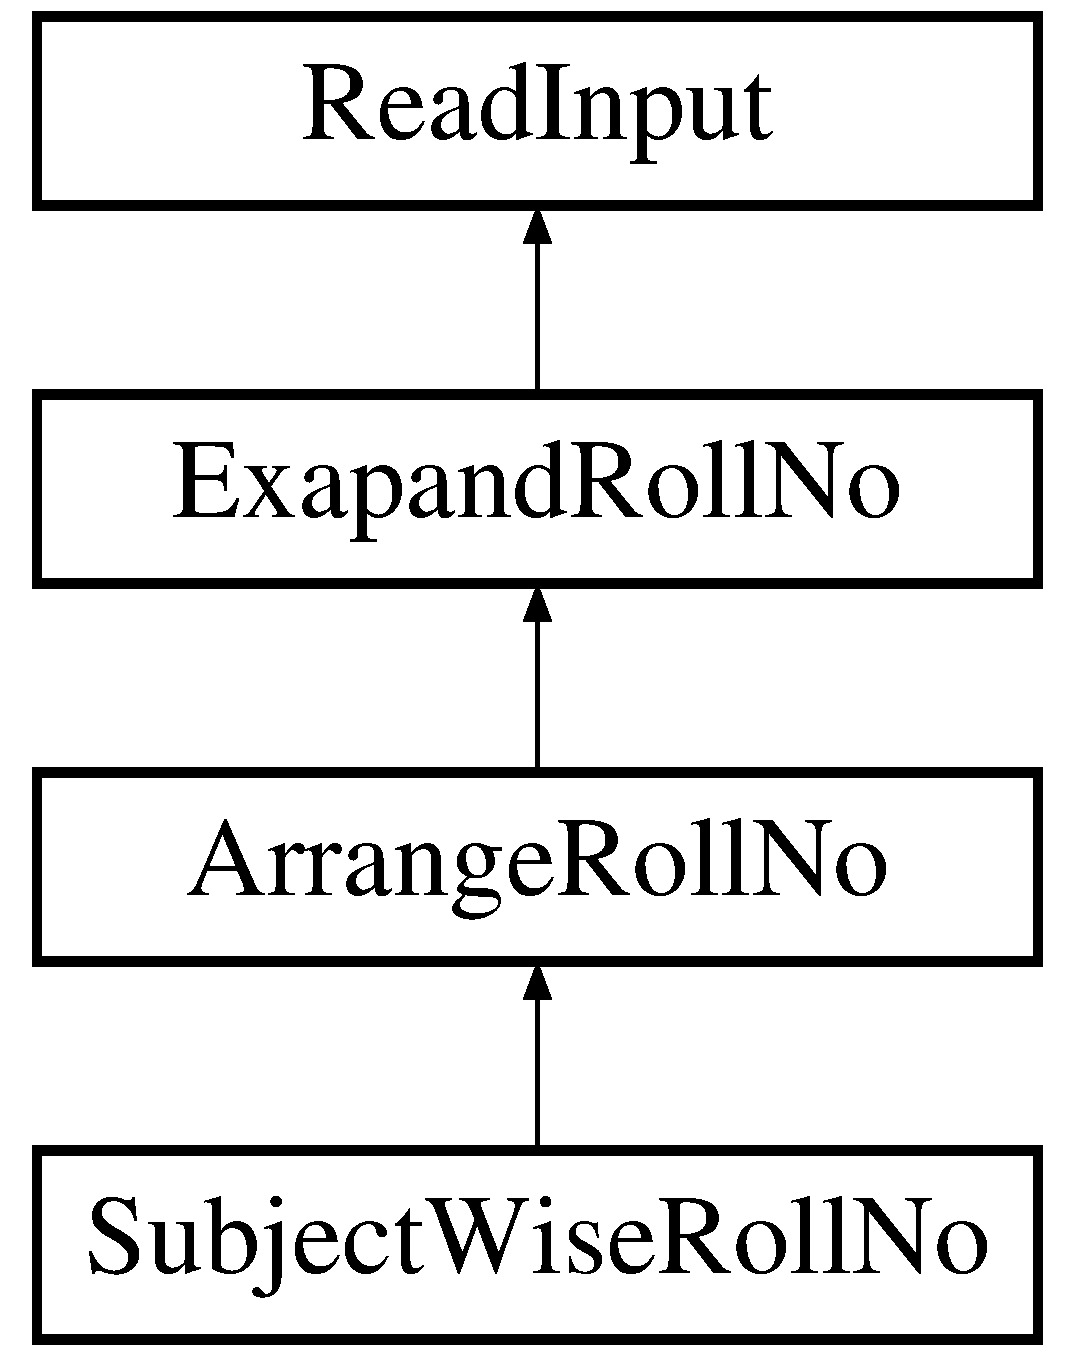
\includegraphics[height=4.000000cm]{classSubjectWiseRollNo}
\end{center}
\end{figure}
\subsection*{Public Member Functions}
\begin{DoxyCompactItemize}
\item 
\hypertarget{classSubjectWiseRollNo_aface8a14361aeeb9a6127d98d60e7732}{void {\bfseries subject\-Wise\-Roll\-No} ()}\label{classSubjectWiseRollNo_aface8a14361aeeb9a6127d98d60e7732}

\item 
\hypertarget{classSubjectWiseRollNo_a243121bce1807bada075e686f740643f}{void {\bfseries set\-Sub\-Code} ()}\label{classSubjectWiseRollNo_a243121bce1807bada075e686f740643f}

\item 
\hypertarget{classSubjectWiseRollNo_acfe5a3d07cad3397efd866fb87b54db7}{void {\bfseries remove\-Redundant\-Sub\-Code} ()}\label{classSubjectWiseRollNo_acfe5a3d07cad3397efd866fb87b54db7}

\item 
\hypertarget{classSubjectWiseRollNo_adb376b81d6b5005889653332a064c977}{void {\bfseries show\-Subject\-Wise\-Roll\-No} ()}\label{classSubjectWiseRollNo_adb376b81d6b5005889653332a064c977}

\item 
\hypertarget{classSubjectWiseRollNo_aeeb07726ddfc0ec17fa8a02c5cd2ffff}{void {\bfseries Main} ()}\label{classSubjectWiseRollNo_aeeb07726ddfc0ec17fa8a02c5cd2ffff}

\end{DoxyCompactItemize}
\subsection*{Protected Attributes}
\begin{DoxyCompactItemize}
\item 
\hypertarget{classSubjectWiseRollNo_aa719b1f10268b6cc741132aced93a321}{int {\bfseries total\-\_\-code}}\label{classSubjectWiseRollNo_aa719b1f10268b6cc741132aced93a321}

\item 
\hypertarget{classSubjectWiseRollNo_a9700a22dff37ac2fd095cbcc3f3e2874}{int {\bfseries sub\-\_\-totalrno} \mbox{[}M\-I\-N\-\_\-\-S\-I\-Z\-E\mbox{]}}\label{classSubjectWiseRollNo_a9700a22dff37ac2fd095cbcc3f3e2874}

\item 
\hypertarget{classSubjectWiseRollNo_a9eef1e17ae0aace37af78b15395ee3e5}{int {\bfseries subject\-\_\-size}}\label{classSubjectWiseRollNo_a9eef1e17ae0aace37af78b15395ee3e5}

\item 
\hypertarget{classSubjectWiseRollNo_a3e21660fe01181bf4595c4fe2163c528}{string {\bfseries sub\-\_\-subcode} \mbox{[}M\-I\-N\-\_\-\-S\-I\-Z\-E\mbox{]}}\label{classSubjectWiseRollNo_a3e21660fe01181bf4595c4fe2163c528}

\item 
\hypertarget{classSubjectWiseRollNo_a20ba02f66c6a634c1f4daeb0bd27b481}{string {\bfseries sub\-\_\-rollno} \mbox{[}M\-I\-N\-\_\-\-S\-I\-Z\-E\mbox{]}\mbox{[}M\-A\-X\-\_\-\-S\-I\-Z\-E\mbox{]}}\label{classSubjectWiseRollNo_a20ba02f66c6a634c1f4daeb0bd27b481}

\end{DoxyCompactItemize}


The documentation for this class was generated from the following files\-:\begin{DoxyCompactItemize}
\item 
Baka\-Plan/\-Seat\-Plan/subject-\/wise-\/rollno.\-h\item 
Baka\-Plan/\-Seat\-Plan/subject-\/wise-\/rollno.\-cc\end{DoxyCompactItemize}

\printindex
\end{document}
